\chapter{Overall Description} \label{cap:cap2}
\section{System Environment}
WeatherCal is a stand alone software made from scratch. It is a Web application that allows the registered users to manage their schedule basing on the weather conditions. The users are also able to invite people to their event and to publicize their event.  
The system is even capable of notifying the users, as they log on to the system, if the weather forecast for the event is not the desired one.
The target of this software is, therefore, to give the users a tool for schedule their events smartly, giving the possibility to change preferences as the weather forecast changes.
\subsection{Actors}
Actors in the system are mainly the people registered into the web application. They will be referred as Registered Users.
Whoever is not yet registered on the platform will be an actor for the system too and it will be identified as an Anonymous  Users.
No administration is required since the system is not intended for illicit purposes and this is a policy of the platform, plus no conflict among users can occur since the only allowed interactions are the invite to an event and a participation to an event (in which other people partecipate).
\subsection{Scenarios}
\begin{itemize}
\item Maggie creates an event for her daughter's birthday, which will be in their garden. She invites all her friends telling them to join the event on WeatherCal to be sure that the forecast will be graceful for that day. Three days before the birthday, Maggie logs in two days before the event and she discovers it will be cloud but she still hopes it won't rain on that day. The day before the event Judith, Maggie's friend, is notified that it could be rainy for the birthday as she logs into the system. Anyway Maggie decides she won't posticipate the birthday. In the end that day was rainy, except for the afternoon, exactly for the birthday, and everything went fine.
\item John wants to go cycling but right now the forecast is not so optimistic, so he decides to use WeatherCal to find the best day for doing so. The platform suggests him that he should go on Monday afternoon, so he plans to do that. Saturday he logs in and discovers that it will be windy on Monday, infact the system suggests him to go cycling on Wednesday and John chooses to do what the system suggests him. In the end he went cycling and the weather was perfect.
\item Beth wants to have a picnic with her friends in two weeks, so she creates an event on WeatherCal when the temperature should be the hottest and there should be no clouds in the sky. Three days before she logs in discovering that for the next two weeks there will be bad weather conditions. She decides so to invite her friends at home for having a launch together.
\end{itemize}
\section{Functional Requirements}
The system allows the users to partecipate in various scenarios:
\begin{itemize}
\item Log on to and log out from the platform.
\item Create, Modify, Delete an event.
\item Invite other users.
\item Manage invitation (accept, refuse).
\item Manage event visibility (decide if an event's infos should be accessible only by its participants). 
\item View other users' profiles.
\end{itemize}
The system is the leading actor in:
\begin{itemize}
\item {Warn all the participants to an event which will occur the following day that there will be bad weather conditions.} 
\item Notify to an event's owner three day before the scheduled data that there will be bad conditions for it suggesting the closest available sunny day.
\end{itemize}
The Anonymous Users are only able to:
\begin{itemize}
\item Sign Up in to the Platform.
\end{itemize}
\section {Goals}
The WeatherCal system should offer and fulfill these main features:
\begin{itemize}
\item A simple management for the users' agendas
\item A swift way to schedule an event according to the weather forecast 
\item Invite other registered users to an event
\item Preserve the privacy of the users since only the user himself can make their info visibile to everyone.
\end{itemize}
\section{Non Functional Requirements}
\subsection{User Interfaces}
The WeatherCal system is a Web application intended to be used trough desktop device.  Its interface is designed in a simple way so that  the user can either easily understand what the system can offer to him and reachs all the main features of the system from a unique view.\\
Once that a user logs in to the system trough a defined web page he is redirected to the main page. This page is divided in two portion. The left one, which occupies most of the page, displays a monthly calendar in which the user manages its events while the right one shows the weather forecast for the following days and also shows the closest events.\\In the figure~\ref{fig:mockup} is shown a first sketch of the main user's page.\\ \\  
 \begin{center}
 \begin{figure}
    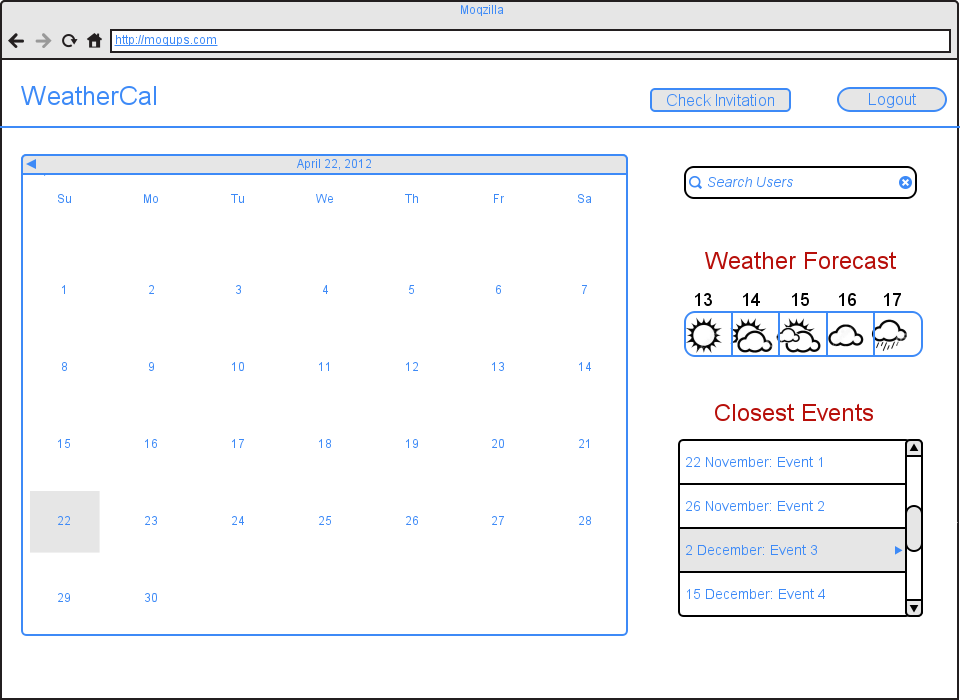
\includegraphics[width=0.9\textwidth]{immagini/UserPage.png}
    \caption{Main Page's MockUp}
     \label{fig:mockup}
     \end{figure}
    \end{center}
\subsection{Performance}
The system offers the users the possibility to use it without major slowdowns. Multiuser usage is allowed and it can be bore by the server application under reasonable conditions, basing on the server hardware.
\subsection{Security}
The system relies on HTTP protocol for transferring data over the Internet, so information sent both from the user to the server and vice-versa will be exposed to possible man-in-the-middle attacks. Unless this issue data stored on the server will be accessible only if valid credentials are provided and there is no possibility for a user to bypass privacy constraints, i.e. users will not be able to see non-public events of other users and modify events for which they are not owners.

